% !TeX program = pdflatex
\documentclass[border=6pt]{standalone}
\usepackage{amsmath}
\usepackage{tikz}
\usetikzlibrary{arrows.meta, positioning, calc, fit, backgrounds}

\definecolor{MediumRed}{rgb}{0.925, 0.345, 0.345}
\definecolor{MediumGreen}{rgb}{0.37, 0.7, 0.66}
\definecolor{MediumBlue}{rgb}{0.015, 0.315, 0.45}
\definecolor{DarkBlue}{rgb}{0.05, 0.15, 0.35}

\begin{document}
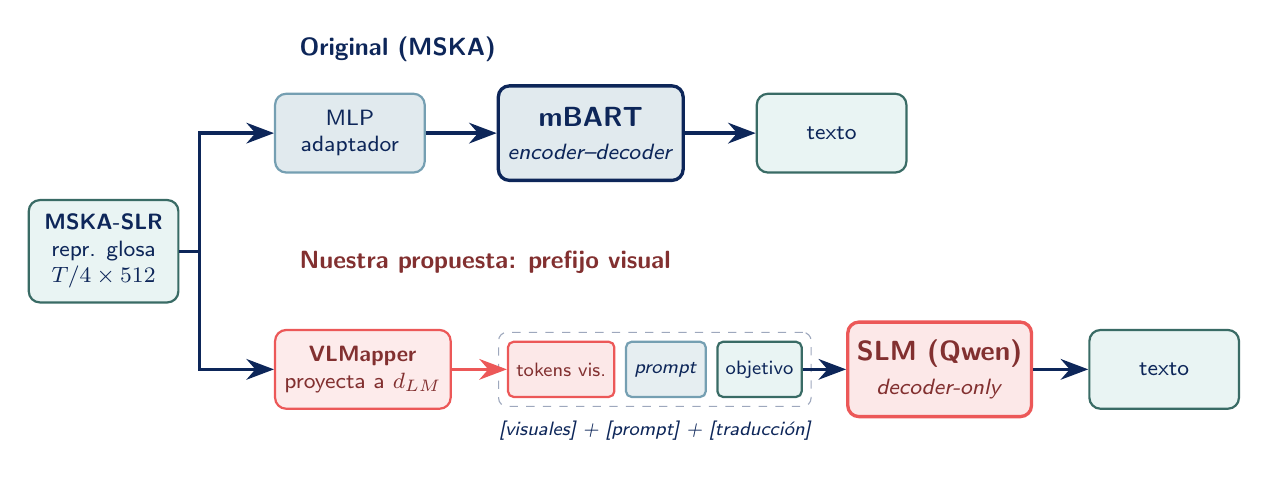
\begin{tikzpicture}[
    font=\sffamily,
    flow/.style={-{Stealth[length=3.5mm]}, line width=1.2pt, DarkBlue},
    blk/.style={draw=MediumBlue!55, thick, rounded corners=4pt, fill=MediumBlue!12,
        text=DarkBlue, align=center, minimum width=1.9cm, minimum height=1.0cm,
        font=\sffamily\footnotesize},
    dec/.style={draw=DarkBlue, very thick, rounded corners=4pt, fill=MediumBlue!16,
        text=DarkBlue, align=center, minimum width=2.2cm, minimum height=1.2cm},
    tok/.style={draw, thick, rounded corners=2pt, minimum height=0.7cm, inner sep=3pt,
        font=\sffamily\scriptsize},
]

% fuente comun
\node[blk, fill=MediumGreen!14, draw=MediumGreen!60!black, minimum height=1.3cm] (glosa)
    at (0,-1.3) {\textbf{MSKA-SLR}\\\footnotesize repr. glosa\\ $T/4\times512$};

% ================= ARRIBA: mBART original =================
\node[blk, right=1.2cm of glosa, yshift=1.5cm] (mlp) {MLP\\\footnotesize adaptador};
\node[dec, right=0.9cm of mlp, fill=MediumBlue!12] (mbart)
    {\textbf{mBART}\\\footnotesize \textit{encoder--decoder}};
\node[blk, right=0.9cm of mbart, fill=MediumGreen!14, draw=MediumGreen!60!black] (txt1) {texto};
\draw[flow] (glosa.east)  -- ++(0.25,0) |- (mlp.west);
\draw[flow] (mlp) -- (mbart);
\draw[flow] (mbart) -- (txt1);
\node[font=\sffamily\small\bfseries, text=DarkBlue] at ($(mlp.north west)+(0.2,0.55)$) [anchor=west]
    {Original (MSKA)};

% ================= ABAJO: SLM decoder-only =================
\node[blk, right=1.2cm of glosa, yshift=-1.5cm, draw=MediumRed, fill=MediumRed!12,
      text=MediumRed!55!black] (vlm) {\textbf{VLMapper}\\\footnotesize proyecta a $d_{LM}$};

% secuencia de prefijo visual
\node[tok, draw=MediumRed, fill=MediumRed!14, text=MediumRed!55!black, right=0.7cm of vlm] (tv) {tokens vis.};
\node[tok, draw=MediumBlue!55, fill=MediumBlue!10, text=DarkBlue, right=0.12cm of tv] (tp) {\textit{prompt}};
\node[tok, draw=MediumGreen!60!black, fill=MediumGreen!14, text=DarkBlue, right=0.12cm of tp] (tt) {objetivo};

\node[dec, right=0.55cm of tt, draw=MediumRed, fill=MediumRed!14, text=MediumRed!55!black,
      minimum width=2.0cm] (slm) {\textbf{SLM (Qwen)}\\\footnotesize \textit{decoder-only}};
\node[blk, right=0.7cm of slm, fill=MediumGreen!14, draw=MediumGreen!60!black] (txt2) {texto};

\draw[flow] (glosa.east) -- ++(0.25,0) |- (vlm.west);
\draw[flow, MediumRed] (vlm) -- (tv);
\draw[flow] (tt) -- (slm);
\draw[flow] (slm) -- (txt2);
\node[font=\sffamily\small\bfseries, text=MediumRed!55!black] at ($(vlm.north west)+(0.2,0.85)$) [anchor=west]
    {Nuestra propuesta: prefijo visual};

% caja alrededor de la secuencia
\begin{scope}[on background layer]
    \node[draw=DarkBlue!40, dashed, rounded corners=3pt, fit=(tv)(tt), inner sep=3pt] (seq) {};
\end{scope}
\node[font=\sffamily\scriptsize\itshape, text=DarkBlue, below=0.05cm of seq]
    {[visuales] + [\textit{prompt}] + [traducción]};

\end{tikzpicture}
\end{document}
